    \item Using Proposition~\ref{prop:copy.tensor}~(items 4 and 5), we can see that 
    $\vb\hadam\ub=$
         \begin{tikzpicture}[baseline=\baseline]
    \tikzset{tensor/.style = {minimum size = 0.5cm,shape = circle,thick,draw=black,inner sep = 0pt}, edge/.style   = {thick,line width=.4mm},every loop/.style={}}
    \def\y{0}
    \def\x{0}
    \draw  node[fill = black,circle,inner sep=0pt,minimum size=4pt] (m) at (\x+0.5,\y+0.5) {};
    \node[tensor,fill=blue!20!red!40!white] (v) at (\x,\y-0.65){\scalebox{0.85}{$\vb$}};
    \node[tensor,fill=red!20!blue!40!white] (u) at (\x+1,\y-0.65){\scalebox{0.85}{$\ub$}};

    \draw[edge] (m) -- (\x,\y) -- (v); 
    
    \draw[edge] (m) -- (\x+1,\y) -- (u); 
    \draw[edge](m) -- (\x+0.5,\y+1);
    \end{tikzpicture}
    $=\text{diag}(\vb)\ub$
\end{itemize}
\end{remark}
To conclude this chapter, we introduce several useful results in the next section.

\subsection{Some Useful Properties of Tensor Networks}\label{sec:useful-TNs}
In this section, we list several useful results about tensor networks. 

\paragraph{Bounding the Rank of Matricizations.}
Any tensor network structure induces a collection of upper bounds on the matricizations of the underlying tensor. More precisely, for an arbitrary tensor network, the rank of a given matricization is bounded by the weight of any cut separating the row legs from the column legs in the graph. Here, the weight of a cut refers to the product of the dimensions of the edges that form the cut. This is formalized in the following theorem. 

\begin{theorem}(Rank of matricization of TN)\label{thm: matricization-rank}
Let $\T \in \Rbb^{d_1\times d_2\times \dots \times d_p}$ be given as a tensor network, and let $I \subset [p]$. Then, for any cut $\mathcal{C}$ separating the legs corresponding to indices in $I$ from the ones in $[p] \setminus I$ in the TN,
$$\rank(\T_{(I)}) \leq \prod_{e \in  \mathrm{cutset}(\mathcal C)} \mathrm{dim}(e),$$
where $\mathrm{cutset}(\mathcal{C})$ is the cut-set\footnote{Formally, the TN is a graph $G=(V,E)$. Each dimension of $\Tt$ is associated with one vertex in $V$: the one to which the corresponding dangling leg is attached. Any cut of this graph $\mathcal C$ is a partition of $V$: $\mathcal{C} = (V_1, V_2)$. In the theorem, we consider cuts that separate indices in $I$ from the other ones, i.e. such that $I \subseteq V_1$~(and thus $([p]\setminus I) \subseteq V_2$ since $(V_1,V_2)$ is a partition of $V$). The cut-set of $\mathcal{C}$ is the set of edges that have one endpoint in $V_1$ and one in $V_2$: $\mathrm{cutset}(\mathcal{C}) = \{(u,v) \in E \mid u\in V_1, v\in V_2 \}$. } %
of $\mathcal C$ and $\mathrm{dim}(e)$ is the dimension of the edge $e$ in the tensor network.
\end{theorem}
Let us illustrate this theorem with some examples. First, we can obtain the classical bound on the rank of a product of matrices as a particular case. Let   $\Ab\in\Rbb^{m\times R}$ and $\Bb\in\RR^{R\times n}$. For the matrix~(i.e., second-order tensor) $\mat{AB} \in \Rbb^{m \times n}$, the theorem gives us the bound

$$\rank(\Ab\Bb)=\rank
\left(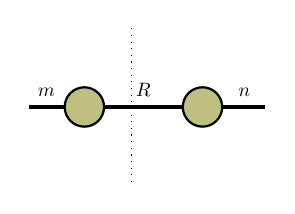
\begin{tikzpicture}[baseline=-0.5ex]
    \tikzset{tensor/.style = {minimum size = 0.5cm,shape = circle,thick,draw=black,inner sep = 0pt}, edge/.style = {thick,line width=.4mm},every loop/.style={}}
    \def\x{6}
    \def\y{0} \node[tensor,fill=green!50!red!50!white] (A) at (\x+1,\y) {$\Ab$};
    \node[tensor,fill=green!50!red!50!white] (B) at (\x+2.5,\y) {$\Bb$};
    \draw[edge] (A) -- (\x+0.3,0) node [midway,above] {\scalebox{0.7}{\dimcolor{$m$}}};
    \draw[edge] (A) -- (B)node [above,midway] {\scalebox{0.7}{\dimcolor{$R$}}};;
    \draw[edge] (B) -- (\x+3.3,\y) node [midway,above] {\scalebox{0.7}{\dimcolor{$n$}}};
    \draw[dotted] (\x+1.6,\y+1) -- (\x+1.6,\y-1);
\end{tikzpicture}\right)\leq R.$$

Now consider the following tensor network representation of a $d_1\times d_2$ matrix:
$$
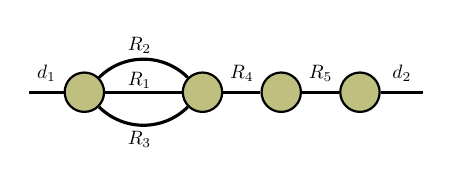
\begin{tikzpicture}[baseline=-0.5ex]
    \tikzset{tensor/.style = {minimum size = 0.5cm,shape = circle,thick,draw=black,inner sep = 0pt}, edge/.style = {thick,line width=.4mm},every loop/.style={}}
    \def\x{6}
    \def\y{0} \node[tensor,fill=green!50!red!50!white] (T) at (\x+1,\y) {$\Tt$};
    \node[tensor,fill=green!50!red!50!white] (A) at (\x+2.5,\y) {$\At$};
    \node[tensor,fill=green!50!red!50!white] (B) at (\x+3.5,\y) {$\Bb$};
      \node[tensor,fill=green!50!red!50!white] (S) at (\x+4.5,\y) {$\Sb$};
    \draw[edge] (T) -- (\x+0.3,\y)node [midway,above] {\scalebox{0.7}{\dimcolor{$d_1$}}};
     \draw[edge] (T) -- (A);
    \draw[edge] (A) -- (B)node [midway,above] {\scalebox{0.7}{\dimcolor{$R_4$}}};
    \draw[edge] (T) to [out=-45,in=-135] (A);
    \draw[edge] (T) to [out=45,in=135] (A);
    \node[draw=none] () at (\x+1.7,\y+0.15) {\scalebox{0.7}{\dimcolor{$R_1$}}};
    \node[draw=none] () at (\x+1.7,\y+0.6) {\scalebox{0.7}{\dimcolor{$R_2$}}};
    \node[draw=none] () at (\x+1.7,\y-0.6) {\scalebox{0.7}{\dimcolor{$R_3$}}};
    \draw[edge](B) -- (S) node [midway,above] {\scalebox{0.7}{\dimcolor{$R_5$}}};
    \draw[edge] (S) -- (\x+5.3,\y) node [midway,above] {\scalebox{0.7}{\dimcolor{$d_2$}}};
    \end{tikzpicture}$$
where $\Tt\in\RR^{d_1\times R_1\times R_2\times R_3}$, $\At\in\RR^{R_1\times R_2\times R_3\times R_4}$, $\Bb\in\RR^{R_4\times R_5}$ and $\Sb\in\RR^{R_5\times d_2}$.
Theorem~\ref{thm: matricization-rank} can for example be used to obtain the upper bounds
$$
\rank\left(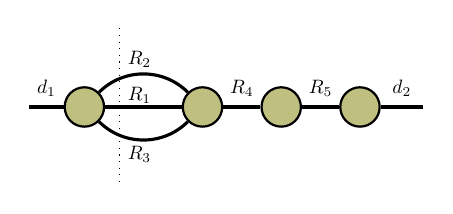
\begin{tikzpicture}[baseline=-0.5ex]
    \tikzset{tensor/.style = {minimum size = 0.5cm,shape = circle,thick,draw=black,inner sep = 0pt}, edge/.style = {thick,line width=.4mm},every loop/.style={}}
    \def\x{6}
    \def\y{0} \node[tensor,fill=green!50!red!50!white] (T) at (\x+1,\y) {$\Tt$};
    \node[tensor,fill=green!50!red!50!white] (A) at (\x+2.5,\y) {$\At$};
    \node[tensor,fill=green!50!red!50!white] (B) at (\x+3.5,\y) {$\Bb$};
      \node[tensor,fill=green!50!red!50!white] (S) at (\x+4.5,\y) {$\Sb$};
    \draw[edge] (T) -- (\x+0.3,\y)node [midway,above] {\scalebox{0.7}{\dimcolor{$d_1$}}};
     \draw[edge] (T) -- (A);
    \draw[edge] (A) -- (B)node [midway,above] {\scalebox{0.7}{\dimcolor{$R_4$}}};
    \draw[edge] (T) to [out=-45,in=-135] (A);
    \draw[edge] (T) to [out=45,in=135] (A);
    \node[draw=none] () at (\x+1.7,\y+0.15) {\scalebox{0.7}{\dimcolor{$R_1$}}};
    \node[draw=none] () at (\x+1.7,\y+0.6) {\scalebox{0.7}{\dimcolor{$R_2$}}};
    \node[draw=none] () at (\x+1.7,\y-0.6) {\scalebox{0.7}{\dimcolor{$R_3$}}};
    \draw[edge](B) -- (S) node [midway,above] {\scalebox{0.7}{\dimcolor{$R_5$}}};
    \draw[edge] (S) -- (\x+5.3,\y) node [midway,above] {\scalebox{0.7}{\dimcolor{$d_2$}}};
    \draw[dotted] (\x+1.45,\y+1) -- (\x+1.45,\y-1);
    \end{tikzpicture}\right)\leq R_1R_2R_3$$
and
$$
\rank
\left(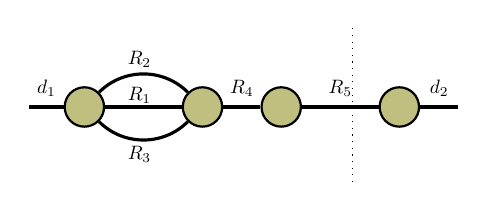
\begin{tikzpicture}[baseline=-0.5ex]
    \tikzset{tensor/.style = {minimum size = 0.5cm,shape = circle,thick,draw=black,inner sep = 0pt}, edge/.style = {thick,line width=.4mm},every loop/.style={}}
    \def\x{6}
    \def\y{0} \node[tensor,fill=green!50!red!50!white] (T) at (\x+1,\y) {$\Tt$};
    \node[tensor,fill=green!50!red!50!white] (A) at (\x+2.5,\y) {$\At$};
    \node[tensor,fill=green!50!red!50!white] (B) at (\x+3.5,\y) {$\Bb$};
      \node[tensor,fill=green!50!red!50!white] (S) at (\x+5,\y) {$\Sb$};
    \draw[edge] (T) -- (\x+0.3,\y)node [midway,above] {\scalebox{0.7}{\dimcolor{$d_1$}}};
     \draw[edge] (T) -- (A);
    \draw[edge] (A) -- (B)node [midway,above] {\scalebox{0.7}{\dimcolor{$R_4$}}};
    \draw[edge] (T) to [out=-45,in=-135] (A);
    \draw[edge] (T) to [out=45,in=135] (A);
    \node[draw=none] () at (\x+1.7,\y+0.15) {\scalebox{0.7}{\dimcolor{$R_1$}}};
    \node[draw=none] () at (\x+1.7,\y+0.6) {\scalebox{0.7}{\dimcolor{$R_2$}}};
    \node[draw=none] () at (\x+1.7,\y-0.6) {\scalebox{0.7}{\dimcolor{$R_3$}}};
    \draw[edge](B) -- (S) node [midway,above] {\scalebox{0.7}{\dimcolor{$R_5$}}};
    \draw[edge] (S) -- (\x+5.75,\y) node [midway,above] {\scalebox{0.7}{\dimcolor{$d_2$}}};
    \draw[dotted] (\x+4.4,\y+1) -- (\x+4.4,\y-1);
    \end{tikzpicture}\right)\leq R_5.
$$
As a final example, let $\Gt\in\RR^{R_1\times\cdots\times R_4}$, $\Ab_1\in\RR^{R_1\times d_1}, \Ab_2\in\RR^{R_2\times d_2},\Ab_3\in\RR^{R_3\times d_3}$ and $\Ab_4\in\RR^{R_4\times d_4}$ and consider the tensor $\T = \Gt \times_1 \Ab_1\times_2 \Ab_2\times_3 \Ab_3\times_4 \Ab_4$. Theorem~\ref{thm: matricization-rank} can be used for example to obtain an upper bound on the rank of the first matricization of $\Tt$:
$$
\rank(\Tt_{(1)}) = 
\rank\left(
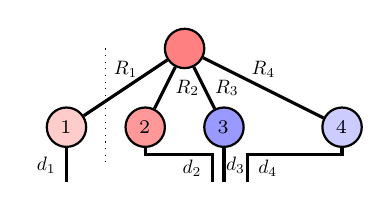
\begin{tikzpicture}[baseline=-0.5ex]
    \tikzset{tensor/.style = {minimum size = 0.5cm,shape = circle,thick,draw=black,inner sep = 0pt}, edge/.style = {thick,line width=.4mm},every loop/.style={}}
    \def\x{6}
    \def\y{0} 
    \node[tensor,fill=red!50!white] (G) at (\x+4.5,\y+1) {$\Gt$};
    \node[tensor,fill=red!20!white] (A_1) at (\x+3,\y){$\Ab_1$};
    \node[tensor,fill=red!40!white] (A_2) at (\x+4,\y){$\Ab_2$};
    \node[tensor, fill=blue!40!white] (A_3) at (\x+5,\y){$\Ab_3$};
    \node[tensor,fill=blue!20!white] (A_4) at (\x+6.5,\y){$\Ab_4$};
    \draw[edge] (G) -- (A_1) node [midway, above] {\scalebox{0.7}{\dimcolor{$R_1$}}};
    \draw[edge] (G) -- (A_2) node [midway, right] {\scalebox{0.7}{\dimcolor{$R_2$}}};
    \draw[edge] (G) -- (A_3) node [midway, right] {\scalebox{0.7}{\dimcolor{$R_3$}}};
    \draw[edge] (G) -- (A_4) node [midway, above] {\scalebox{0.7}{\dimcolor{$R_4$}}};
    \draw[edge] (A_1) -- (\x+3,\y-0.7) node [midway, left] {\scalebox{0.7}{\dimcolor{$d_1$}}};
    \draw[edge] (A_3) -- (\x+5,\y-0.7) node [midway, right=-0.11cm] {\scalebox{0.7}{\dimcolor{$d_3$}}};
    \draw[edge] (A_2) -- (\x+4,\y-0.35) -- (\x+4.85,\y-0.35) -- (\x+4.85,\y-0.7) node [midway, left] {\scalebox{0.7}{\dimcolor{$d_2$}}};
    \draw[edge] (A_4) -- (\x+6.5,\y-0.35) -- (\x+5.30,\y-0.35) -- (\x+5.30,\y-0.7) node [midway, right] {\scalebox{0.7}{\dimcolor{$d_4$}}};
    \draw[dotted](\x+3.5,\y+1)-- (\x+3.5,\y-0.5);
    \end{tikzpicture}\right)\leq R_1.
$$
\paragraph{TN Edges and Sum Tensors.}Let $\T$ be a tensor given as a TN. Any edge in which the TN corresponds to one way to express the tensor as a sum of tensors of the same size as $\T$. This follows directly from the definition of edges in TNs. An edge represents a contraction, which is a sum. We illustrate this concept with examples. First, consider a rank-$R$ factorization of an $m\times n$ matrix. The edge in the TN corresponds to expressing the matrix as a sum of $R$ (rank-one) matrices:  
$$
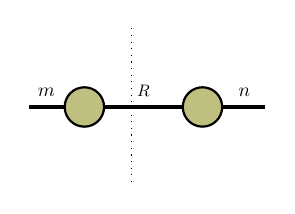
\begin{tikzpicture}[baseline=-0.5ex]
    \tikzset{tensor/.style = {minimum size = 0.5cm,shape = circle,thick,draw=black,inner sep = 0pt}, edge/.style = {thick,line width=.4mm},every loop/.style={}}
    \def\x{6}
    \def\y{0} \node[tensor,fill=green!50!red!50!white] (A) at (\x+1,\y) {$\Ab$};
    \node[tensor,fill=green!50!red!50!white] (B) at (\x+2.5,\y) {$\Bb$};
    \draw[edge] (A) -- (\x+0.3,0) node [midway,above] {\scalebox{0.7}{\dimcolor{$m$}}};
    \draw[edge] (A) -- (B)node [above,midway] {\scalebox{0.6}{\dimcolor{$R$}}};;
    \draw[edge] (B) -- (\x+3.3,\y) node [midway,above] {\scalebox{0.7}{\dimcolor{$n$}}};
    \draw[dotted] (\x+1.6,\y+1) -- (\x+1.6,\y-1);
\end{tikzpicture}
= 
\sum_{r=1}^R
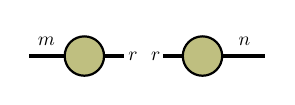
\begin{tikzpicture}[baseline=-0.5ex]
    \tikzset{tensor/.style = {minimum size = 0.5cm,shape = circle,thick,draw=black,inner sep = 0pt}, edge/.style = {thick,line width=.4mm},every loop/.style={}}
    \def\x{6}
    \def\y{0} \node[tensor,fill=green!50!red!50!white] (A) at (\x+1,\y) {$\Ab$};
    \node[tensor,fill=green!50!red!50!white] (B) at (\x+2.5,\y) {$\Bb$};
    \draw[edge] (A) -- (\x+0.3,0) node [midway,above] {\scalebox{0.7}{\dimcolor{$m$}}};
    \draw[edge] (A) -- (\x+1.5,\y) node [pos=1.5] {\scalebox{0.7}{\indcolor{$r$}}};
    \draw[edge] (B) -- (\x+3.3,\y) node [midway,above] {\scalebox{0.7}{\dimcolor{$n$}}};
    \draw[edge](B) -- (\x+2,\y)node [pos=1.4] {\scalebox{0.7}{\indcolor{$r$}}};
\end{tikzpicture}
= \sum_{r=1}^R \Ab_{:,r} \Bb_{r,:} = \sum_{r=1}^R \ab_r \outprod \bb_r,
$$
where $\ab_r$ are the columns of $\Ab\in\RR^{m\times R}$ and $\bb_r$ are the rows of $\Bb\in\RR^{R\times n}$.

